% Thesis template, taken from CVPR 2022 paper template.
% CVPR 2022 Paper Template
% based on the CVPR template provided by Ming-Ming Cheng (https://github.com/MCG-NKU/CVPR_Template)
% modified and extended by Stefan Roth (stefan.roth@NOSPAMtu-darmstadt.de)

\documentclass[10pt,twocolumn,letterpaper]{article}

%%%%%%%%% PAPER TYPE  - PLEASE UPDATE FOR FINAL VERSION
%\usepackage[review]{sarmata}      % To produce the REVIEW version
\usepackage{sarmata}              % To produce the CAMERA-READY version
%\usepackage[pagenumbers]{cvpr} % To force page numbers, e.g. for an arXiv version

% Include other packages here, before hyperref.

\usepackage{multirow}
\usepackage{graphicx}
\usepackage{amsmath}
\usepackage{amssymb}
\usepackage{booktabs}
\usepackage[pagebackref,breaklinks,colorlinks]{hyperref}
\usepackage[none]{hyphenat}
% Support for easy cross-referencing
\usepackage[capitalize]{cleveref}
\crefname{section}{Sec.}{Secs.}
\Crefname{section}{Section}{Sections}
\Crefname{table}{Table}{Tables}
\crefname{table}{Tab.}{Tabs.}


\begin{document}

\begin{titlepage}
    \begin{center}
        % Logos
        
\includegraphics[width=0.3\textwidth]{hhu_logo.png} \hfill \\[1cm]

        {\Large\textsc{Heinrich-Heine-Universität D\"usseldorf}}\\[3cm]
        {\Large\textbf{Bachelor Thesis}}\\[1cm]

        {\Huge\textbf{Game Playing Agents MicroRTS}}\\[2cm]

        {\Large\textbf{{Maximilian Huft}}}\\[2cm]

        \vfill
        % Details
        \begin{tabbing}
            \hspace{4cm} \= \hspace{8cm} \= \\ % Tab stops
            Degree: \> B.Sc. Computer Science \\
            Supervisor: \> Professor Dr. Paul Swoboda \\
            Co-Supervisor: \> Dr. Peter Arndt \\
            Faculty: \> Faculty of Mathematics and Natural Sciences \\
        \end{tabbing}

        \vfill % Vertical space

        {\large 22.08.2025}
    \end{center}
\end{titlepage}

%%%%%%%%% ABSTRACT
\begin{abstract}
Real-time strategy (RTS) games are a challenging domain for deep reinforcement learning (DRL) due to large action spaces and delayed rewards. This thesis investigates the development of a competitive agent for the MicroRTS environment capable of consistently defeating the built-in scripted bots. The training pipeline combines behavior cloning (BC) to learn an initial policy from expert replays with Proximal Policy Optimization (PPO) for subsequent policy refinement.  

Empirical results show that BC provides a robust initialization, while PPO fine-tuning further improves performance through exploration and adaptation. Together, these methods yield faster convergence and stronger policies than either approach alone. The resulting agent achieves strong win rates across a variety of built-in opponents in fewer than 30 million steps, demonstrating the effectiveness of combining imitation learning and deep reinforcement learning for RTS domains.
\end{abstract}


\tableofcontents
\newpage

%%%%%%%%% BODY TEXT´
\section{Introduction}
\label{sec:intro}

Modern video games offer researchers complex and diverse environments for developing and evaluating deep reinforcement learning (DRL) agents. Among these, real-time strategy (RTS) games have become a particularly important genre for AI research. They combine challenges such as large and variable action spaces, real-time decision-making constraints, and the need for concurrent strategic reasoning under continuous time pressure~\cite{ontanon2013survey}. RTS environments, unlike turn-based games such as Chess or Go, require agents to manage multiple interdependent tasks simultaneously. These tasks include actions spanning over long stretches of time, like resource collection, as well as actions that require tactical planning and adaptation to the opponent’s behavior, such as unit production and building construction. There are also challenges that demand high precision, where queuing an action just one timestep too late can determine the outcome of the entire match, such as in combat and unit movement. The complexity is further increased by different unit types with distinct strengths and weaknesses, actions that can involve controlling multiple entities at once, and nondeterministic elements that may influence outcomes. Furthermore, partial observability limits the information available about the opponent’s state, necessitating active scouting and exploration of the map, while the diversity of map layouts and sizes demands varied strategic adaptations. In addition, reward signals are often sparse and delayed until the end of a match, potentially thousands of timesteps after key decisions were made, making effective reward assignment particularly challenging. These characteristics collectively make RTS games a valuable and demanding testbed for evaluating approaches that integrate long-horizon planning, uncertainty handling, and real-time reactive control.

MicroRTS is a simplified yet still challenging RTS environment, designed specifically for AI research and benchmarking~\cite{huang2021gym}. Unlike large-scale commercial titles such as StarCraft, MicroRTS offers a lightweight implementation with minimal engineering overhead, while retaining the core difficulties that make RTS games challenging for artificial intelligence. In particular, it features a large action space where agents must issue commands to multiple units simultaneously and partial observability through Fog of War. These properties require agents to integrate tactical reasoning while adapting in real time to an opponent’s actions. Furthermore, the environment includes nondeterministic elements and diverse opponent strategies, which emphasize the need for robustness and generalization. This makes it an ideal platform for exploring new approaches to agent design without the heavy engineering and computational burden of a full-scale game.

In this work, two learning approaches are explored: behavior cloning (BC) and Proximal Policy Optimization (PPO)\footnote{\href{https://github.com/mahuf100/MicroRTS_Maximilian_Huft}{https://github.com/mahuf100/MicroRTS\_Maximilian\_Huft}}. BC is a form of imitation learning where an agent learns to replicate expert behavior by training on recorded demonstrations, enabling it to quickly acquire a competent baseline policy~\cite{torabi2018behavioral}. PPO is a DRL algorithm that improves an agent’s policy by interacting with the environment and maximizing expected rewards, while maintaining stability through clipped policy updates~\cite{schulman2017ppo}. While BC can rapidly produce reasonable performance, it is limited by the quality and diversity of the expert data. PPO, on the other hand, can surpass expert performance through exploration, but it often struggles with sparse rewards and poor initial performance~\cite{martin2021beclone}. Combining BC and PPO leverages the strengths of both methods using BC to bootstrap initial competence and PPO to refine the agent through exploration.

The goal of this thesis is to develop a MicroRTS agent that can consistently defeat the built-in scripted bots, which serve as a strong and diverse baseline. By combining BC with DRL, this hybrid pipeline not only accelerates training but also yields a competitive agent that achieves high win rates even against the strongest built-in opponents.


\section{Related Work}
\label{sec:related-work}

\noindent\textbf{MicroRTS-Py (Gym-MicroRTS)}  
\cite{huang2021gym} introduced MicroRTS-Py, an OpenAI Gym wrapper for MicroRTS, which includes a PPO~\cite{schulman2017ppo} implementation that was trained on the \texttt{basesWorkers16x16A} map. In their work, they explored many techniques and different approaches to improve their agent. Their best performing approach incorporated action composition, a shaped reward function, invalid action masking, and the IMPALA-CNN~\cite{espeholt2018impala} architecture with residual blocks~\cite{he2016deep}. Training was conducted against a diverse set of scripted agents, resulting in a 91\% win rate on the target map against competition-level bots.   Ablation studies revealed that invalid action masking was critical, its removal reduced the win rate to 0\%. Additionally, in their paper "Comparing Observation and Action Representations for DRL in MicroRTS" they compared two action-generation strategies: Unit Action Simulation (UAS), which calls the policy sequentially for each unit and simulates intermediate states, and GridNet, which computes actions for all units in a single pass using per-grid-position logits and a player action mask~\cite{huang2020observation}. UAS achieved slightly higher performance (91\% vs. 89\%), but due to its complexity and limited compatibility with self-play and imitation learning, they decided to focus on GridNet and deprecated UAS.

They demonstrated that PPO with invalid-action masking and grid-wise action representations serves as a strong baseline for MicroRTS. Their work is widely used as a foundation in MicroRTS-based research and their  gridnet\_diverse\_impala  agent served as a baseline for this thesis.


\vspace{10pt}


\noindent\textbf{RAISocketAI}
RAISocketAI won the IEEE-CoG 2023 MicroRTS competition, becoming the first DRL agent to claim the title in the competition’s six-year history~\cite{goodfriend2024raisocketai}. It consistently outperformed previous champions, setting a new performance benchmark for DRL in MicroRTS. Its success was driven by iteratively fine-tuning the base policy and their training schedule. They also used different network architectures depending on the map size and applied transfer learning from agents trained on smaller maps to agents designed for larger maps to reduce training time. Additionally, after creating their competition winning agent, they also experimented with incorporating BC demonstrating its effectiveness as a pretraining method for improving DRL initiation and the resulting  boost to training speed.

Beyond the competition results, RAISocketAI contributed several enhancements to the MicroRTS-Py framework, including bug fixes and new functionality for recording bot-vs-bot replays. This replay recording capability allowed the creation of the demonstration dataset used for BC in this thesis.
\vspace{10pt}

\noindent\textbf{BeClone}
BeClone demonstrated that combining BC with DRL fine-tuning can effectively improve agent performance in real-time strategy games, specifically in MicroRTS~\cite{martin2021beclone}. Their approach follows a two-phase training process: first, BC is used with expert demonstration data to train a base policy, allowing the agent to achieve initial competence without relying on environment reward signals. Second, the policy is refined through using an Advantage Actor-Critic (A2C) algorithm, enabling dynamic strategy adaptation and more effective exploration. This method was used to create several bots for different map sizes with the goal of maximizing resource-gathering. The resulting agents outperformed the baseline agent from Huang and Ontañón~\cite{huang2021gym} in both reward performance and training efficiency.

While experiments were restricted to resource-gathering tasks on small maps (maximum size $8 \times 8$), the results indicate that BC followed by DRL fine-tuning is a promising approach for MicroRTS and potentially other RTS domains.
\vspace{10pt}

\noindent\textbf{AlphaStar}
\cite{vinyals2019sc2} released AlphaStar, a grandmaster-level AI for StarCraft II trained using DRL. The system was initially bootstrapped with imitation learning sampling replays of the top-quartile of human players. The resulting supervised agents performed in the top 16\% of human players and served as the starting point for DRL training. AlphaStar was trained using a self-play league in which a continuously evolving population of agents, including main competitors, exploiters, and past versions, trained against each other to enhance strategic robustness and prevent forgetting.
Compared to StarCraft II, MicroRTS is far simpler in both complexity and simulation cost. The action and observation spaces also differ substantially between the two environments. In StarCraft’s learning environment, AlphaStar’s actions consist of: selecting an action type, selecting a subset of units and  choosing a target. Once issued, these actions are executed until completion or interruption. In contrast, MicroRTS  requires issuing discrete, single-step actions for each unit at every timestep.
Despite the differences in scale, complexity, and computational resources available to DeepMind, AlphaStar served as a conceptual inspiration and informed several design and implementation choices in the development of the MicroRTS agent.




\section{Method}
\label{sec:method}

\subsection{Environment Setup}
\label{sec:env-setup}

All experiments were conducted in the MicroRTS environment using RAISocketAI’s reimplementation of MicroRTS-Py~\cite{goodfriend2024raisocketai}. All training and evaluations were performed on the \texttt{basesWorkers16x16A} map, commonly used in the MicroRTS research community~\cite{huang2021gym,ontanon2018first}. The map contains a player base, an enemy base, a single initial worker for each player, and 4 resource patches, 2 per player. A screenshot of the game is shown in Figure~\ref{Figure 1}. Green square tiles indicate resource nodes, with the overlaid numbers denoting remaining resources. Units outlined in blue belong to player~1, while units outlined in red belong to player~2. Light-gray square icons represent bases, and darker-gray squares denote barracks. Movable units are represented as circles. Small gray circles denote workers, which have low health and attack damage but can construct buildings and gather resources. Orange circles represent light units, which are fast moving with low health but relatively high attack damage. Blue circles indicate ranged units, which have low health and low attack damage but can attack enemies from up to three squares away. Yellow circles represent heavy units, which have high health and high attack damage. The unit types also differ in cost and production time. Workers cost only 1 and are produced quickly. Light and ranged units cost 2 and have medium production times. Heavy units cost 3 and require significantly longer to produce. The unit interactions follow a rock–paper–scissors relationship where: light units are effective against ranged units, ranged units are effective against heavy units, and heavy units are effective against light units~\cite{richoux2020microphantom}.
Partial observability (Fog of War) was disabled to simplify learning and provide the agent with the full game state at all times. The maximum episode length was set to 2,000 game steps. This limit was chosen because most matches on this map finish before the 2000-step mark, while those that do not typically take significantly longer to conclude.

 The environment provides observations in the form of a channel-based spatial representation. The observation tensor has the shape \((T, N, H, W, C)\), where:
\begin{itemize}
    \item \(T\) — number of timesteps in the sequence
    \item \(N\) — number of parallel environments
    \item \(H\) — map height 
    \item \(W\) — map width (usually the same as map height)
    \item \(C\) — number of feature channels (73 in this environment)
\end{itemize}

Each feature channel encodes a specific aspect of the game state, such as unit type, hit points, ownership, resource amounts, and production status. Since partial observability is disabled, these observations represent the complete game state at every step. In practice, the CNN backbone processes tensors of shape \((B, 73, 16, 16)\), where the batch dimension is defined as \(B = T \times N\), flattening the temporal and environment axes.

The action space follows a multi-discrete per-tile encoding. Actions are represented as a tensor of shape \((T, N, H \times W, A)\), where \(A = 7\) is the number of discrete action components. The seven independent discrete subactions are: action type, move direction, harvest direction, return direction, produce direction, produce type and relative attack position. For each tile on the map, the agent specifies a 7-dimensional action vector covering these subactions. Correspondingly, the actor head outputs logits of shape \((16 \times 16 \times 78)\), where the 78 dimensions arise from the expanded parameterization of the seven subactions. For example, the subaction "move direction" requires four discrete logits (north, south, east, west), while "produce type" requires one logit per unit type. Together, the concatenation of all subaction options yields 78 logits per tile, ensuring consistency between the per-tile multi-discrete encoding and the network’s output.

To improve training efficiency, invalid action masking was applied to restrict the policy’s choices to only valid actions for the current state. Invalid action masking is applied by setting the corresponding logits to a very large negative value, effectively assigning zero probability and gradient to actions that are illegal or have no effect (e.g., moving a unit that does not exist). This masking substantially reduces the effective action space per turn, improving training efficiency~\cite{huang2020invalid}.

To incorporate information about the source of demonstrations, during BC, the agent converts the expert’s name into a learned embedding \(z\), while simultaneously encoding the current observation using an observation encoder to produce its own estimate of the expert embedding. These two representations are combined using a blending factor \(\alpha\). Early in training, \(\alpha \approx 1\), so the agent relies primarily on the expert-provided \(z\). Over 30 epochs, \(\alpha\) linearly decreases to zero, gradually shifting the agent’s reliance toward the observation-based encoding. This allows the encoder to learn associations between gameplay patterns and expert identity. In subsequent PPO training, the observation encoder alone determines \(z\), ensuring the network can both leverage multiple expert styles and adapt to new situations.

In addition, a scalar feature vector is extracted from the observation to capture global game statistics, similar to the scalar features used in~\cite{vinyals2019sc2}. This scalar vector contains 11 features:
\begin{itemize}
    \item Player 0 stored resources
    \item Player 1 stored resources
    \item Available resources left on the map
    \item Player 0: number of workers, light units, heavy units, ranged units
    \item Player 1: number of workers, light units, heavy units, ranged units
\end{itemize}
These features are processed by a dedicated encoder before being concatenated with \(z\) and the CNN backbone features.


\begin{figure}[h]
    \centering
    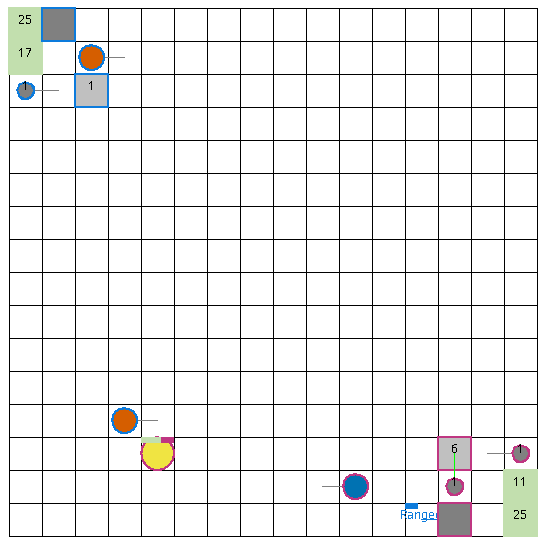
\includegraphics[width=1\linewidth]{images/16x16.png}
    \caption{Screenshot of the MicroRTS \texttt{basesWorkers16x16A} map, including all units and buildings. }
    \label{Figure 1}
\end{figure}

\subsection{Neural Network Architecture}


\label{sec:nn-architecture}

The agent’s policy and value networks share a common convolutional backbone and separate linear heads for actor and critic. The backbone (Figure~\ref{Figure 2}) processes the input observation tensor of shape \((B, 73, 16, 16)\) and produces a 256-dimensional feature representation for each batch element, resulting in an output tensor of shape \((B, 256)\).

It uses residual connections implemented as residual blocks (ResBlocks) ~\cite{he2016deep}. The ResBlocks apply two $3\times3$ convolutions with padding $1$: the first convolution is followed by a GELU activation, while the second is followed by a Squeeze-and-Excitation (SE) block. The SE block compresses each channel via global average pooling. Then the pooled vector goes through a bottleneck $1\times1$ convolution that reduces channel dimensionality by a factor of 16, followed by a GELU activation. After the original channel dimensionality is restored with a second $1\times1$ convolution and a sigmoid activation to produce channel-wise weights. The output of the second convolution is reweighted by these channel weights and added to the original input via a residual connection and a final GELU activation is applied to the sum. This design enables the block to extract local spatial features, dynamically emphasize informative channels, and improve gradient flow for stable training of deeper networks.

Two auxiliary encoding modules are used alongside the convolutional backbone: a scalar feature encoder that compresses global, non-spatial game statistics into a fixed-size vector, and a zEncoder that produces a compact latent conditioning vector from the observations.
\paragraph{ScalarEncoder}  
The ScalarEncoder is a small multi-layer perceptron that maps a compact set of global game statistics to a feature vector used by both actor and critic. It consists of \(L=2\) fully connected layers. The first layer projects the input of dimension \(d_{\text{in}}\) to a hidden layer of width 32 with ReLU activation, and the second maps this hidden vector to an output space of dimension 32:
\[
\mathrm{ScalarEncoder}:\ \mathbb{R}^{d_{\text{in}}}\rightarrow\mathbb{R}^{d_{\text{out}}},
\]
In this implementation \(d_{\text{in}}=11\) and \(d_{\text{out}}=32\). This dense representation summarizes global information such as resources and unit counts into a compact form that complements spatial features extracted by the convolutional backbone. It provides both actor and critic networks with access to global context, improving strategic decision-making beyond purely spatial information.

\paragraph{zEncoder.}  
The zEncoder is a lightweight feed-forward network that maps the current observation into a compact latent code \(z\). It is implemented as a two-layer perceptron with an intermediate hidden size of 64 and a ReLU activation in between them:
\[
\mathrm{zEncoder}:\ \mathbb{R}^{d_{\text{obs}}}\rightarrow\mathbb{R}^{d_z},
\]

In this work the flattened observation dimension \(d_{\text{obs}}=16\times16\times73\), and the latent dimension \(d_{\text{z}}=8\). This structure provides a dense, low-dimensional summary of the observation. During the BC phase, the output is combined with an expert-provided embedding via a blending schedule, allowing the zEncoder to learn associations between gameplay patterns and expert identity.  This enables the policy to exploit diverse expert behaviors during BC while retaining the flexibility to generalize.
\vspace{10pt}
The ScalarEncoder supplies explicit, low-dimensional global statistics that support value estimation and high-level decision making. The zEncoder produces a dense latent conditioning vector that, together with a compact expert identity embedding, enables the policy to represent broader contextual factors. This design allows the agent to condition on demonstration style during BC, thereby capturing different expert playstyles, and later to adapt to varied contexts during PPO fine-tuning.

The ScalarEncoder and zEncoder are concatenated with the CNN-produced spatial feature vector to form the final state representation fed to the actor and critic heads:
\[
h = \big[h_{\text{cnn}} \,\|\, h_{\text{scalar}} \,\|\, h_{z}\big] \in \mathbb{R}^{256+32+8}.
\]

Two separate linear heads, map the concatenated representation \(h\) to policy logits and a scalar state value:

\begin{figure}[h]
    \centering
    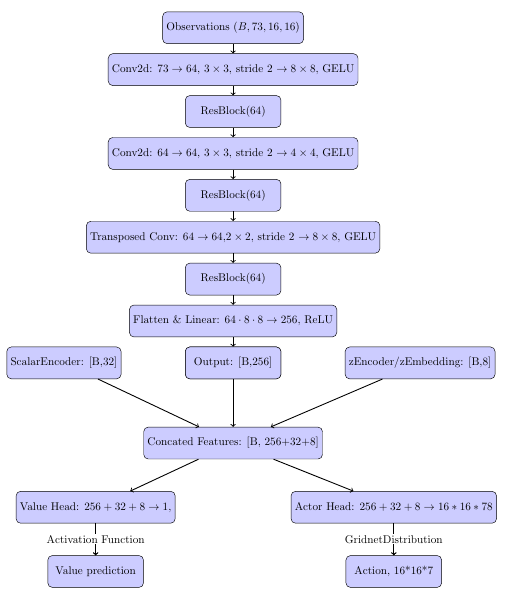
\includegraphics[width=1.1\linewidth, height=10cm]{images/diagram.png}
    \caption{The Network Architecture}
    \label{Figure 2}
\end{figure}

\begin{itemize}
  \item \(\text{actor}(h) = \mathrm{Linear}\big(256+32+8 \rightarrow M\big)\) — produces logits for the multi-discrete per-tile action encoding. In this implementation \(M = \text{mapsize} \times \text{action\_plane\_size} = 16 \times 16 \times 78\) , i.e. a block of logits per map tile covering all action components.
  \item \(\text{critic}(h) = \mathrm{Linear}\big(256+32+8 \rightarrow 1\big)\) — predicts the state value.
\end{itemize}
The layer weights are initialized using orthogonal initialization with a configurable standard deviation, while biases are set to a constant value~\cite{schulman2017ppo}. The actor head uses a small standard deviation (\(0.01\)) to keep initial logits near zero, while the critic uses a larger standard deviation( \(1.0\)).

The architecture incorporates several key design principles that facilitate effective policy learning in the RTS domain.  
First, GELU activations are used throughout the convolutional pathway and within the ResBlocks, while a ReLU activation is applied after the final linear projection of the CNN backbone before concatenation with auxiliary encoders. This combination improves non-linear expressivity while maintaining numerical stability. Residual connections further alleviate vanishing gradients and enable deeper feature processing~\cite{he2016deep}, while SE attention adaptively re-weights channel activations, allowing the network to focus on informative features across different game contexts~\cite{hu2018squeeze}.

To balance efficiency and spatial reasoning, the model employs stride-2 convolutions for downsampling followed by transpose convolutions for upsampling. This reduces computational cost while preserving sufficient spatial context for per-tile action decoding. Beyond spatial features, auxiliary encoders process scalar statistics and a latent variable \(z\), which together supply global, non-spatial, and contextual information that cannot be captured by convolutional processing alone.  

Finally, the policy head implements a per-tile multi-discrete action representation, directly aligned with the environment’s action encoding. This design enables the network to output actions for all map locations in parallel, ensuring efficient and scalable policy execution~\cite{huang2020observation}.




\subsection{Behavior Cloning}
\label{sec:bc}
For the BC phase, expert demonstrations were generated by having the 2020 competition winner CoacAI and the 2021 competition winner Mayari play against all built-in bots in MicroRTS. The bot environment was configured to be nondeterministic, introducing small variations in the replays and thus producing more diverse training data and the maximum amount of timesteps per game was set to 2000. The same number of replays from CoacAI and Mayari was used, with 50 to 300 replays collected per matchup. Harder and more random opponents were prioritized over easier ones, which tend to produce repetitive game states, resulting in a total of 5400 replays comprising approximately 7 million game states.
Additionally, a secondary dataset was collected, filtering for only the games in which the expert won. This resulted in a smaller dataset, containing roughly 4100 games with around 5.2 million game states. This dataset was used for fine-tuning the agent following the initial BC training phase.

The expert observations are fed into the policy network, and the resulting logits are compared to the expert actions to compute the BC loss. The objective function is defined as:

\[
\mathcal{L}_{\text{BC}}(\theta) = - \frac{1}{B \cdot H \cdot W} \sum_{b,h,w} \log \pi_\theta(a^{\text{expert}}_{b,h,w} \mid s_{b,h,w}),
\]

Here $B$ denotes the batch size, $(H,W)$ the map height and width, $s$ the observation, $a^{\text{expert}}$ the expert actions, and $\pi_{\theta}$ the policy with parameters $\theta$. The summation runs over all batch elements $b$ and spatial locations $(h,w)$, i.e., every tile in the input maps. The loss is normalized by the total number of tiles in the batch ($B \cdot H \cdot W$). This per-tile normalization ensures a consistent scaling of the loss across different batch and map sizes



\subsection{Reinforcement Training}

After the BC phase, the supervised policy was further fine-tuned using DRL to improve its performance and adaptability beyond the scope of the expert demonstrations. The PPO algorithm was employed for this stage. The same environment configurations were used to ensure continuity between the BC and RL phases. Two rewards were used during training, a win-loss reward and an attack reward. The win-loss reward is 10 for a win, -10 for a loss and 0 for a draw. This reward is further scaled by a linear function, which is approximately 1.1 at 500 steps and decreases to about 0.9 at 2000 steps. This encourages agents to win games quickly and to prolong games when losing, thereby rewarding faster victories and slower defeats. After BC training, the agent continued to exhibit difficulties in consistently attacking nearby enemy units, either delaying the attack or not attacking at all. To address this, an attack reward was introduced, granting the agent a reward for each valid attack. This attack reward is much smaller than the win-loss reward, set at 0.05 per attack and averages approximately 0.9 reward per game. This reward helps the agent in learning to attack an enemy unit, similar to the  attack reward used in~\cite{goodfriend2024raisocketai}, while still remaining small enough not to interfere with the primary objective of winning the game. Only these two rewards were used, since the agent should already have learned basic MicroRTS mechanics such as resource gathering, unit training, and unit control.

During reinforcement training, the agent was trained against a mix of built-in MicroRTS bots. This training setup encouraged the agent to adapt dynamically to different opponent strategies while exploring parts of the action space~\cite{huang2021gym}.

The policy is trained using the PPO loss function~\cite{schulman2017ppo}:
\begin{equation*}
L(\theta) = \hat{\mathbb{E}}_t \Big[ 
    L^{\text{CLIP}}(\theta) 
    - c_1 L^{\text{VF}}(\theta) 
    + c_2 S\big[\pi_\theta\big](s_t) 
\Big],
\label{eq:ppo_total}
\end{equation*}
where the clipped surrogate objective is

\begin{align*}
L^{\text{CLIP}}(\theta) 
  &= \min \Bigg(
      \frac{\pi_\theta(a_t \mid s_t)}{\pi_{\theta_{\text{old}}}(a_t \mid s_t)} \, \hat{A}_t, \nonumber \\ 
  &\quad \text{clip}\!\left(
        \frac{\pi_\theta(a_t \mid s_t)}{\pi_{\theta_{\text{old}}}(a_t \mid s_t)}, 
        1 - \epsilon, 1 + \epsilon
    \right)\hat{A}_t
  \Bigg).
\end{align*}


and the value function loss is
\begin{equation*}
L^{\text{VF}}(\theta) = \tfrac{1}{2}\,\big( V_\theta(s_t) - \hat{V}_t \big)^2.
\label{eq:ppo_value}
\end{equation*}


where $c_1$ is the value loss coefficient, $c_2$ is the entropy coefficient, $S$ is the entropy bonus function, $\pi_\theta$ is the stochastic policy, $\pi_{\theta_{\text{old}}}$ is the rollout policy, $a_t$ is the action taken at time $t$, $s_t$ is the observation at time $t$, $\hat{A}_t$ is the advantage estimate, $\epsilon$ is the clipping coefficient, $V_\theta$ is the value function, and $\hat{V}_t$ is the return estimate. The advantage is estimated using Generalized Advantage Estimation (GAE)~\cite{schulman2015high}, with hyperparameters $\gamma$ (discount factor) and $\lambda$ (exponential weighting). GAE is employed to reduce the variance of the advantage estimates while introducing only a small bias, which stabilizes policy updates and improves learning efficiency. The resulting advantage estimates are then used in the clipped policy loss $\mathcal{L}_{\text{CLIP}}$.

To prevent the policy from deviating too far from the supervised BC policy, we include a KL divergence regularization term. For each minibatch, the KL divergence is computed between the current policy $\pi_\theta$ and the target supervised policy $\pi_{\text{target}}$ over all per-tile discrete action distributions:

\[
\text{KL}_{\text{div}} = \frac{1}{B} \sum_{b=1}^{B} \text{KL}\Big(\pi_{\text{BC}}^{(b)} \,\|\, \pi_\theta^{(b)} \Big),
\]

where $B$ is the minibatch size. Both $\pi_\theta$ and $\pi_{\text{BC}}$ are obtained by applying the softmax function to the respective logits. The KL divergence is then scaled by a coefficient $\lambda_{\text{KL}}$ and then added to the overall loss. This regularization encourages the learned policy to remain close to the BC policy, stabilizing learning and preventing overconfident deviations during PPO training.

\section{Experiments}
\label{sec:experiments}

\subsection{Setup}
The agent was trained in three sequential stages: BC, BC fine-tuning (BC-FT) and PPO.

The initial BC phase used a total of 5400 replays, generated against the built-in Mayari and CoacAI opponents (see Section~\ref{sec:bc} for replay generation details). Training ran for 100 epochs with the Adam optimizer, an initial learning rate of \(1\times 10^{-3}\), and a batch size of 2048. The BC loss plateaued after 100 epochs, with no further improvement. 
Afterwards, the agent was fine-tuned using another dataset of roughly 4100 replays that only included games where the expert won, with identical optimizer settings and batch size. The model converged within 70 epochs, only requiring roughly half the training time needed during the initial BC phase. During both phases, linear learning rate annealing was used, which proved particularly beneficial, enabling  a higher initial learning rate that accelerated early learning while stabilizing convergence later on. 

\begin{table}[h]
\centering
\caption{Training parameters for PPO training.}
\begin{tabular}{l c}
\hline
\textbf{Parameter} & \textbf{Value} \\
\hline
Initial learning rate (Adam) & $2.5 \times 10^{-5}$ \\
Rollout steps per environment & 512 \\
Minibatch Size & 3072\\
Max episode length & 2,000 timesteps \\
Discount factor $\gamma$ &  1 \\
Value function coefficient $\beta$ & 0.01 \\
Entropy coefficient $\eta$ & 0.005 \\
Gradient norm threshold $\omega$ &0.5 \\
KL regularization coefficient $\lambda_{\text{KL}}$ & 0.4 \\
GAE parameter $\lambda$ & 0.95 \\
\hline
\end{tabular}
\label{tab:training_params}
\end{table} 

The BC-FT policy was further optimized using PPO with 24 parallel game environments. The best performance was achieved when only training against CoacAI and Mayari. 16 CoacAI and 8 Mayari environments were used, based on observations that the agent performed better against Mayari during training. PPO used a rollout size of 512 leading to a total rollout size of 24 $\times$ 512 = 12288 timesteps. Using a larger rollout size compared to~\cite{huang2021gym} proved vital, as rewards in this work were much sparser, focusing mainly on the win-loss reward. Four mini-batches and four PPO updates were used per rollout, resulting in a minibatch size of 3072 and a total of 16 gradient steps per rollout, which allowed the agent to efficiently process experience while stabilizing training. PPO was configured with an initial learning rate of \(2.5\times 10^{-5}\),  \(\lambda_{\mathrm{GAE}}=0.95\), entropy coefficient 0.005, value coefficient 0.01, maximum gradient norm 0.5, clipping coefficient 0.1 and \(\gamma=1.0\) (no discount applied) in order to accurately reflect the true objective of winning games. The learning rate was linearly annealed throughout training to improve convergence and stabilize learning. The parameter values were chosen based on prior work~\cite{goodfriend2024raisocketai, vinyals2019sc2} and through empirical experimentation with different settings. Training was run for 30 million steps, after which both episode reward and win rate plateaued.

At the end of each stage (BC, BC-FT, PPO), a total of 100 deterministic evaluation games were conducted against all built-in bots in MicroRTS. All evaluations were conducted on the \texttt{basesWorkers16x16A} map with both partial observability and nondeterminism disabled.

\begin{table}[ht]
\centering
\caption{Win rates (\%) of BC, BC-FT, and after PPO against each bot.}
\label{tab:winrates_all}
\begin{tabular}{lccc}
\hline
\textbf{Bot} & \textbf{BC} & \textbf{BC-FT} & \textbf{PPO} \\
\hline
WorkerRushAI     & 3 & 50 & 99 \\
PassiveAI        & 98& 100& 100 \\
LightRushAI      & 22 & 93 & 99 \\
CoacAI           & 0 & 8 & 96 \\
Mayari           & 0 & 5 & 95 \\
RandomAI         & 52 & 95 & 99\\
RandomBiasedAI   & 18 & 68 & 86\\
rojo             & 0 & 34& 84 \\
mixedBot         & 4 & 44 & 59 \\
izanagi          & 0& 62& 61\\
tiamat           & 11 & 78& 84 \\
droplet          & 0& 31& 59\\
guidedRojoA3N    & 4 & 42& 75 \\
naiveMCTS      & 0 & 5& 3 \\
\hline
\end{tabular}
\end{table}

\subsection{Results}

We evaluated our agent across three stages: behavior cloning (BC), fine-tuned behavior cloning (BC-FT), and reinforcement learning with Proximal Policy Optimization (PPO). Table~\ref{tab:winrates_all} summarizes overall win rates, showing clear performance improvements across stages.

The initial BC phase produced policies capable of imitating basic expert behaviors, such as resource gathering and unit production, but the agent still struggled with unit control and combat actions. While the agent occasionally defeated weaker bots, it could not consistently secure victories and failed against stronger opponents. 

Fine-tuning on a smaller dataset containing only winning replays led to noticeable improvements. Leveraging the pretrained policy with this focused dataset reduced training time and allowed the agent to reliably defeat weaker bots, though it still rarely overcame stronger adversaries. The resulting agent was able to perform more advanced tasks, such as unit control and combat, but frequent small mistakes and inconsistencies often led to losses against stronger opponents, confirming that imitation learning alone is insufficient for mastering MicroRTS. The overall win rate improved from $20.3\%$ (BC)  to $54.8\%$ (BC-FT).

The largest gains came from PPO training. After fewer than 30 million steps, the agent achieved near-perfect win rates against weaker bots and competitive results against strong opponents such as CoacAI and Mayari. Targeted training on these two bots not only boosted direct performance but also generalized well to other strong bots. Expanding the opponent pool during PPO training decreased performance, emphasizing the importance of opponent selection. During PPO training the overall win rate improved to $88.6\%$. 

The final agent achieved similar or higher win rates than the gridnet\_diverse\_impala agent~\cite{huang2021gym} against most bots. For example, against LightRushAI, the final agent achieved a win rate of 99\%, compared to 79\% for the baseline, and against Izanagi, the final agent achieved 61\% compared to 48\%. Some exceptions were RandomBiasedAI (86\% vs. 100\%), NaiveMCTS (3\% vs. 14\%), rojo (84\% vs. 100\%) and guidedRojoA3N (75\% vs. 91\%). Against CoacAI, the final agent achieved a 96\% win rate, even managing to outperform the RAISocketAI agent’s 90\% win rate on the same map with identical settings~\cite{goodfriend2024raisocketai}. These results were obtained using only 30 million timesteps, compared to the 300 million timesteps required by both the gridnet\_diverse\_impala agent and RAISocketAI.
Despite achieving a high overall win rate, the final agent struggled against highly stochastic bots (Rojo, RandomBiasedAI, NaiveMCTS) where almost all non-wins were draws caused by single units hiding in corners of the map. Attempting to improve performance against these bots by training exclusively against RandomBiasedAI proved ineffective, reducing both the win rate and subsequently episode reward, as shown in Figure~\ref{Figure 4}. 
The agent also demonstrated difficulties in controlling ranged units effectively. Instead of exploiting their longer attack distance, it often moved them into melee range, thereby negating their advantage. As a consequence, the policy tended to favor producing heavy units, which are more robust in close combat. Light units were not used at all, due to the expert demonstrations from CoacAI and Mayari exclusively using heavy and ranged units.

Figure~\ref{Figure 3} shows average win rates during PPO training under different opponent configurations, where training with 16 CoacAI and 8 Mayari yielded the strongest results. 
Extending training beyond 30 million steps yielded no improvement, as seen in Figure~\ref{Figure 3}. Figure~\ref{Figure 4} illustrates that training the final agent on a broader set of opponents also did not  seem to have any significant effect on the win rate, indicating a trade-off between opponent diversity and specialization.

Overall, our results demonstrate that combining BC, targeted fine-tuning, and PPO yields substantial improvements, especially inregards to training time, with opponent selection and learning rate scheduling being critical factors in achieving high performance.



\begin{figure}[h]
    \centering
    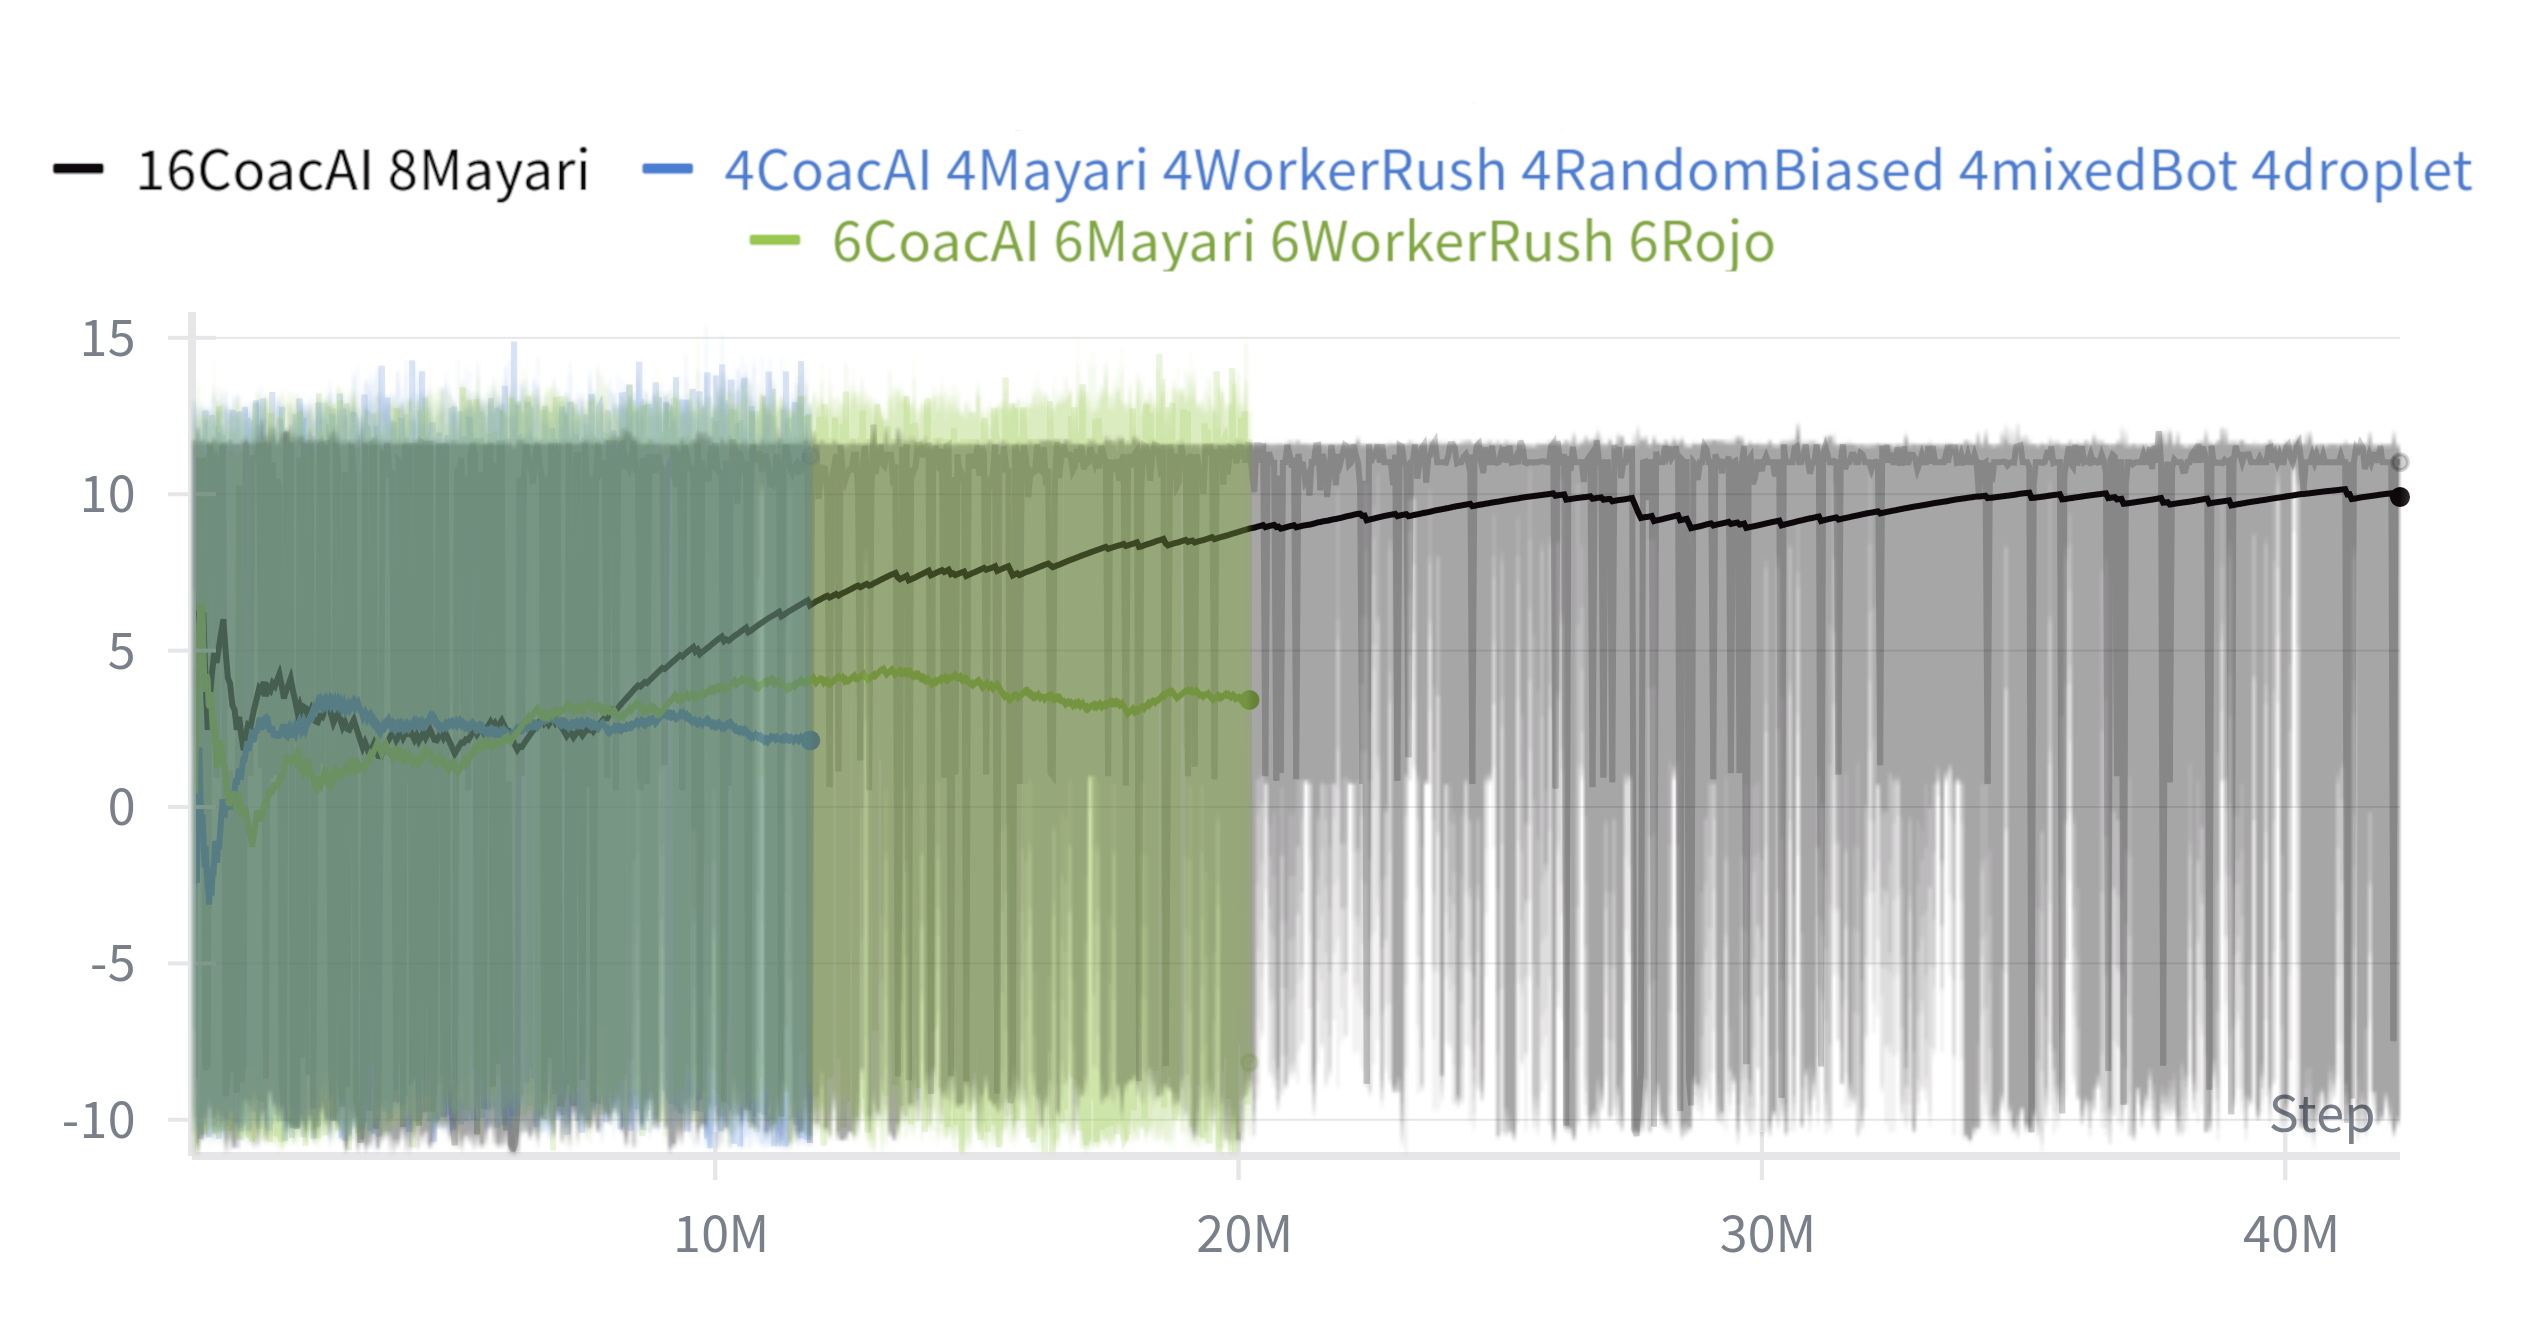
\includegraphics[width=1\linewidth]{images/Fig3.png}
    \caption{Episode rewards (y-axis) as a function of training timesteps (x-axis) on the BC-FT agent.}
    \label{Figure 3}
\end{figure}

\begin{figure}[h]
    \centering
    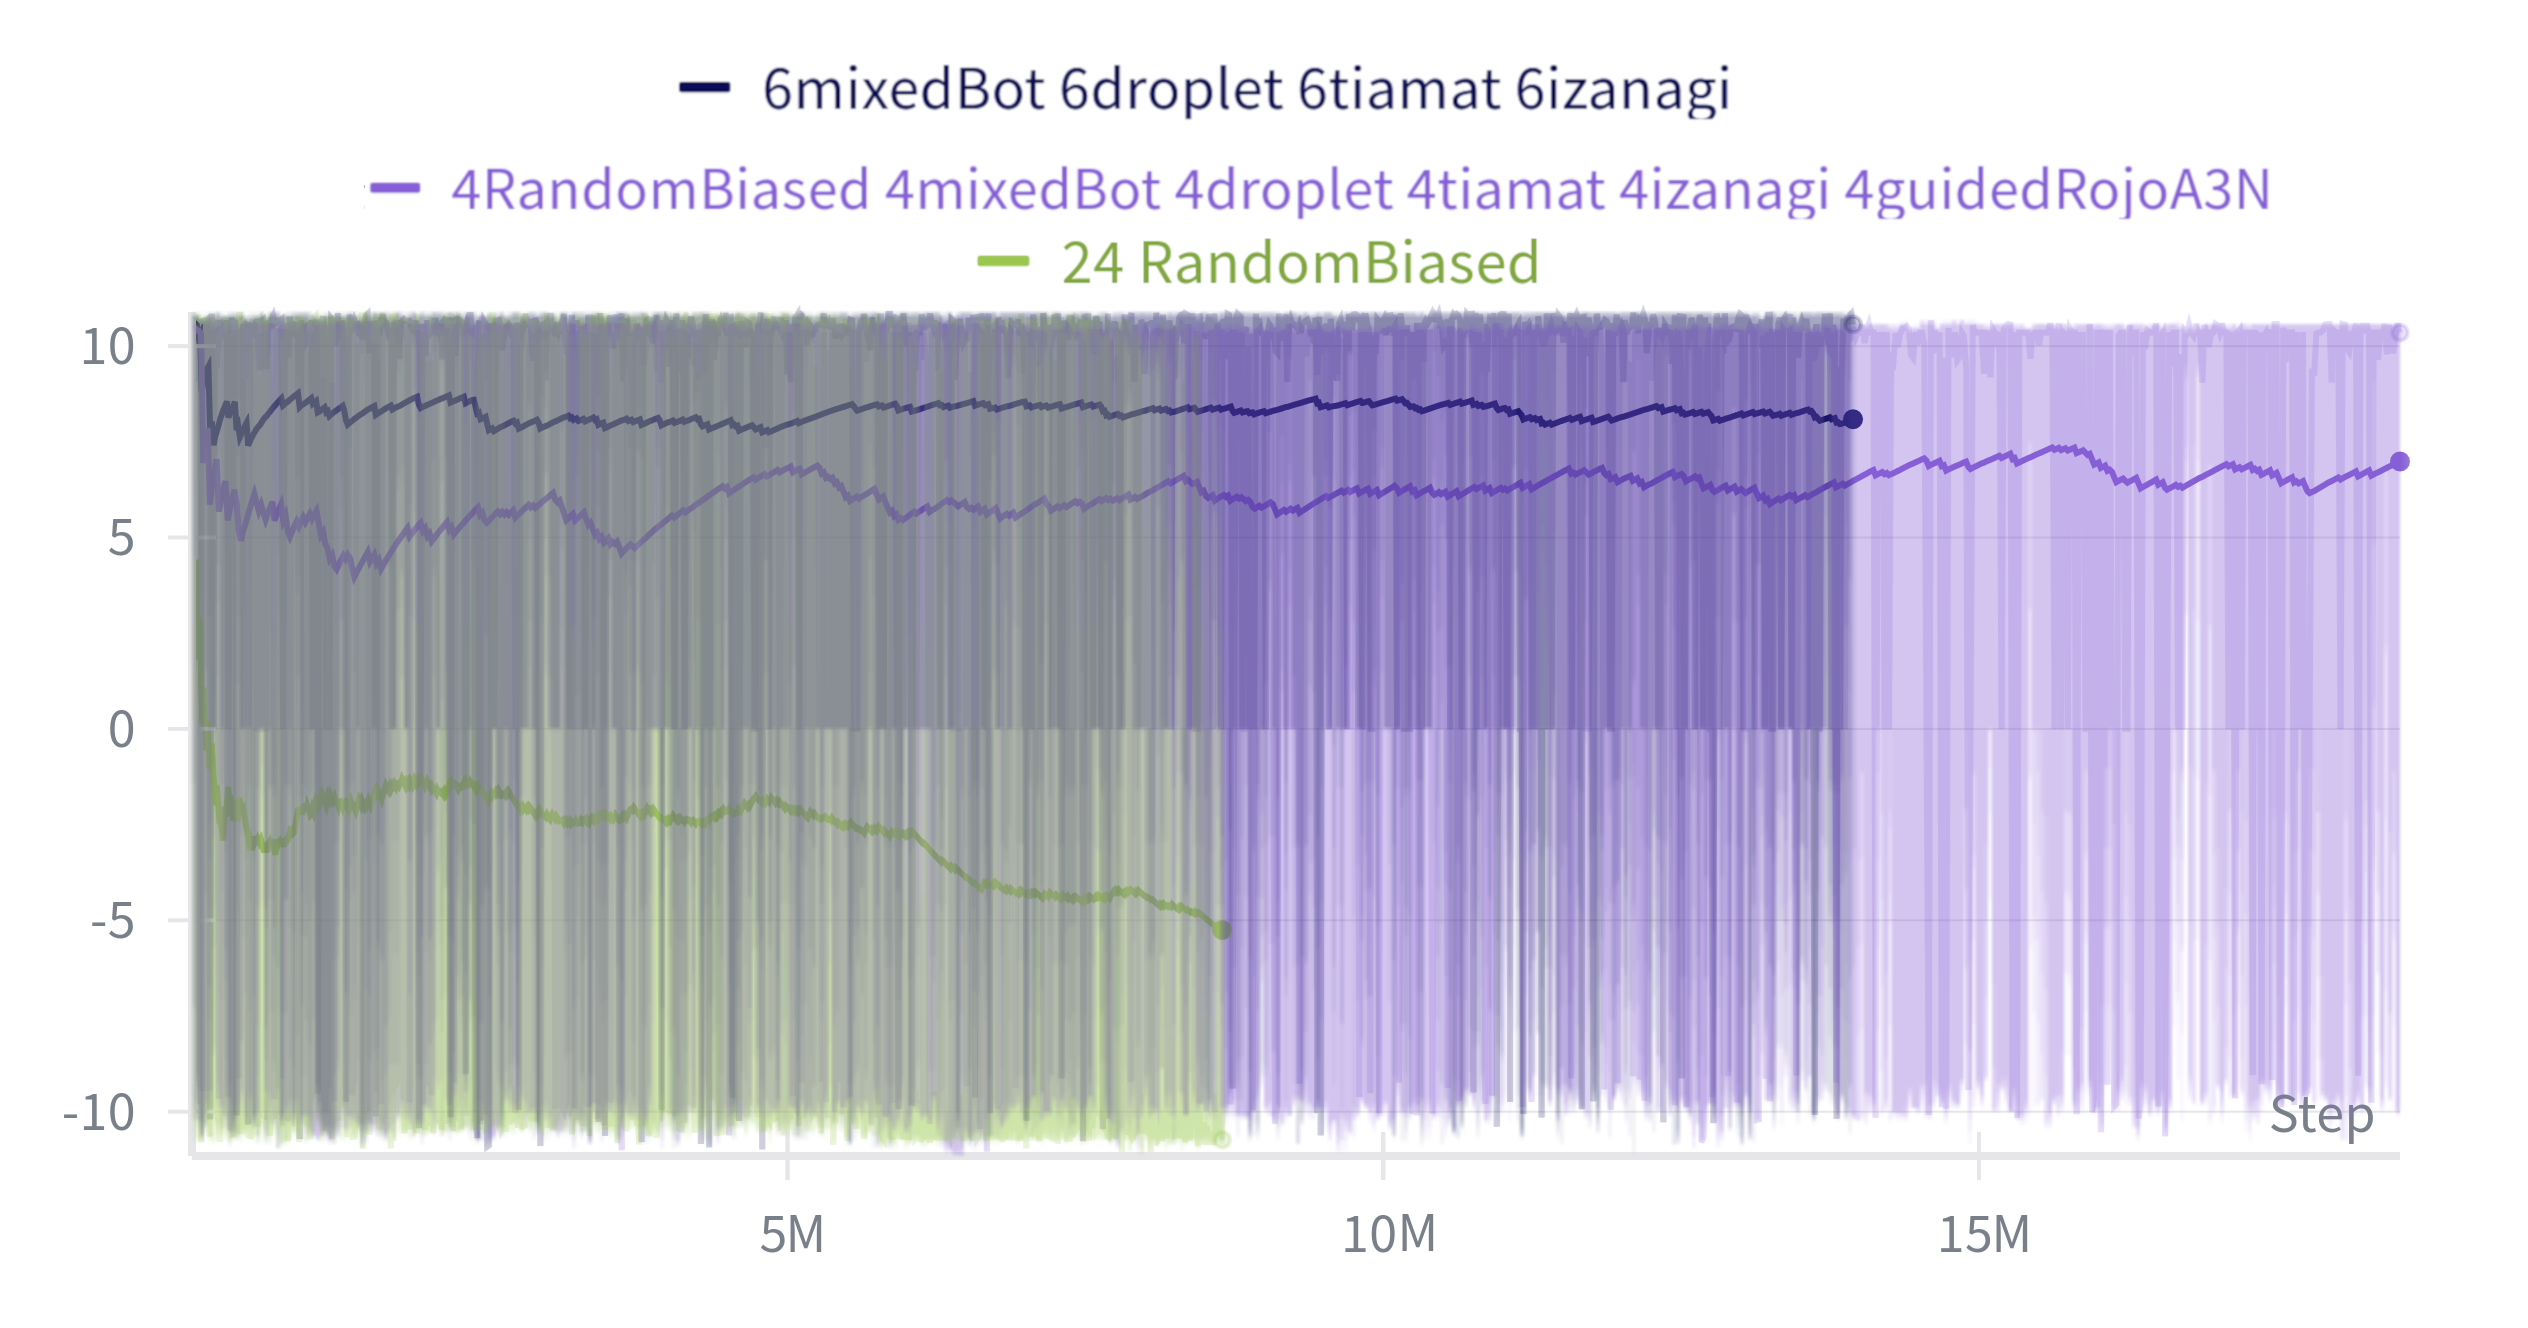
\includegraphics[width=1\linewidth]{images/Fig4.png}
    \caption{Episode rewards (y-axis) as a function of training timesteps (x-axis) on the final agent.}
    \label{Figure 4}
\end{figure}


\subsection{Discussion}

Together, these results highlight the complementary strengths of BC and DRL. BC bootstrapped a competent policy, bypassing the need to learn basic mechanics such as resource gathering and unit production. Fine-tuning the policy on winning replays accelerated the acquisition of higher-level skills, such as coordinated unit control, while also reinforcing the previously learned fundamentals. PPO then refined these policies through exploration and adaptation, achieving near-perfect results against weaker bots and competitive performance against stronger adversaries such as CoacAI and Mayari.

Training exclusively against CoacAI and Mayari not only improved performance against them, but also generalized well to other strong adversaries. Experiments with broader or alternative opponent pools often yielded no improvement and, in some cases, degraded performance. This tension between opponent diversity and specialization reflects a classic bias–variance trade-off where training on a narrow pool risks overfitting to specific strategies, while expanding the opponent set can introduce variance that hinders learning progress. Balancing these competing factors remains a key challenge for scaling to more robust and general policies.

Overall, this hybrid approach demonstrates that BC can rapidly bootstrap policies in complex action spaces, while PPO fine-tunes strategies and adapts to challenging scenarios, highlighting the benefits of targeted opponent selection. 

Despite the overall success, several limitations were identified:  
\begin{itemize}
    \item \textbf{Generalization to random opponents:} The agent struggled with highly random bots such as RandomBiasedAI and NaiveMCTS, where most nonwins were draws caused by a single unit hiding in a corner of the map. This demonstrates that the agent has issues when encountering new or unseen game states.
    \item \textbf{Map and observability constraints:} All experiments were conducted on the \texttt{basesWorkers16x16A} map without partial observability. Scaling to larger maps or Fog of War would require broader and more diverse replay datasets.
    \item \textbf{Replay and training bottlenecks:} Collecting replays and training against compute-heavy bots (e.g.,guidedRojoA3N, NaiveMCTS, Droplet) significantly slowed the process, making it inefficient to train on them.
    \item \textbf{Exploitability:} The agent was trained exclusively using built-in bots and demonstrated limited exposure to new and unexplored game states. As a result, it remains vulnerable to opponents employing unconventional strategies, such as attacking from inefficient routes or deliberately hiding units when losing, which could be easily exploited.
\end{itemize}

Several avenues could extend and improve the current work. Self-play was not utilized in this study to avoid overcomplicating training. However, several studies have demonstrated the benefits of self-play in MicroRTS~\cite{goodfriend2024raisocketai}, \cite{huang2021gym}. Implementing a self-play league system, where different versions of the agent compete against each other and are grouped into distinct agent types, like the approach used in AlphaStar~\cite{vinyals2019sc2}, appears particularly promising for further performance improvements.   Scaling to different maps and exploring different game settings like partial observability turned on need to be addressed before the agent can be considered fully functional. \cite{goodfriend2024raisocketai} showed the potential of using transfer learning to different maps, as well as using different network architectures depending on the size of the map. Expanding the replay dataset with demonstrations that include game states not present in the current dataset, such as starting the expert agent from a disadvantaged position or from positions it would not normally encounter, could improve generalization and robustness. Similarly, incorporating replays from stronger and more diverse opponents, such as other competition winners and participants, could further enhance performance. Investigating persistent points of failure, such as enemy units hiding in corners, by developing strategies or reward shaping to address rare or unexplored game states could improve the agent’s ability to handle such situations. It is also important to note that during the IEEE-CoG MicroRTS competition, agents are limited to 100 ms per timestep. While the current agent does not exceed this limit, future implementations, especially on larger and more complex maps, may require more computation time and risk surpassing the time budget. 


\section{Conclusion}
\label{sec:conclusion}

This thesis presented the development of a competitive MicroRTS agent trained using a combination of behavior cloning and Proximal Policy Optimization. Starting from expert demonstrations, the agent learned to imitate strong play and was subsequently fine-tuned through deep reinforcement learning to adapt and improve in dynamic game situations. The results indicate that while behavior cloning accelerates early-stage training, reinforcement learning remains essential for creating a competitive agent in MicroRTS.

The resulting agent outperformed or achieved comparable performance to existing baselines on most opponents, attaining consistently strong win rates, even against some of the strongest bots, while requiring only a fraction of the training time. Training primarily on winning replays accelerated the acquisition of advanced skills such as unit coordination, tactical combat, and broader strategic decision-making, while the careful selection of challenging opponents promoted generalization to unseen matchups. These results demonstrate that behavior cloning, when combined with PPO fine-tuning, can effectively tackle the large and complex action spaces characteristic of real-time strategy games.

Beyond MicroRTS, this study reinforces the viability of combining imitation learning and reinforcement learning in domains with large action spaces and sparse rewards. These findings may extend to other RTS benchmarks like StarCraft II or to broader sequential decision-making problems with similar characteristics.

Despite these successes, the study was limited to the \texttt{basesWorkers16x16A} map with Fog of War disabled, and opponent diversity during training and evaluation was constrained. Consequently, the agent’s adaptability to larger maps, partially observable settings, or entirely new opponents remains untested. Future work should focus on enabling partial observability, scaling to larger and more diverse maps, increasing opponent diversity, and leveraging advanced demonstration data. Implementing self-play and transfer learning may further enhance robustness and adaptability, while careful attention to computational constraints will ensure feasibility in competition settings. Addressing these areas is essential for developing future agents that are fully competition-ready in MicroRTS.
In summary, this work demonstrates that combining imitation learning with PPO fine-tuning is a powerful paradigm for tackling the challenges of RTS games. By addressing scalability, diversity, and uncertainty, future agents could not only become strong MicroRTS competitors but also contribute to broader progress in creating DRL agents that must plan, act, and learn in complex real-time environments with large action spaces.



%%%%%%%%% REFERENCES
{\small
\bibliographystyle{apalike}
\bibliography{references}
}

%%%%%%%%% Erkl\"arung
\onecolumn
\pagebreak\noindent
\textbf{\LARGE Erkl\"arung}
\addcontentsline{toc}{section}{Erkl\"arung}

\bigskip\bigskip
\noindent 
Hiermit versichere ich, dass ich die   Bachelorarbeit selbst\"andig verfasst und keine
anderen als die angegebenen Quellen und Hilfsmittel benutzt habe.

\bigskip
\noindent
D\"usseldorf, den 22.08.2025

\bigskip\bigskip\bigskip
\noindent
{Maximilian Huft}

\newpage

\end{document}
